%% SoftwareX Original Software Publication: svcc 0.1.0
%% Structure follows the SoftwareX OSP layout (code metadata table C1-C9, sections 1-5).
%% Check against the current SoftwareX template before submission: the guide for
%% authors could not be read from the build machine (ScienceDirect refused the fetch).
\documentclass[preprint,12pt]{elsarticle}

\usepackage[T1]{fontenc}
\usepackage[utf8]{inputenc}
\usepackage{amssymb}
\usepackage{booktabs}
\usepackage{tabularx}
\usepackage{array}
\usepackage{listings}
\usepackage{xcolor}
\usepackage{tikz}
\usetikzlibrary{arrows.meta,positioning}
\usepackage[hyphens]{url}
\usepackage[hidelinks]{hyperref}
\usepackage{microtype}
\setlength{\emergencystretch}{2em}

\lstset{basicstyle=\ttfamily\footnotesize,columns=fullflexible,keepspaces=true,
  frame=single,framerule=0.3pt,rulecolor=\color{black!40},breaklines=true,
  xleftmargin=2pt,xrightmargin=2pt,aboveskip=6pt,belowskip=6pt}
\newcommand{\code}[1]{\texttt{#1}}

\journal{SoftwareX}

\begin{document}

\begin{frontmatter}

\title{svcc: Converting SystemVerilog RTL to SystemC with a Proof for Every Generated Model}

\author{Mayur Kubavat}
\ead{mkubavat01@gmail.com}
\affiliation{organization={Independent Researcher},city={Mountain View},state={CA},country={USA}}

\begin{abstract}
Hardware teams keep C++ and SystemC models of their register-transfer level (RTL) designs for
virtual platforms, software bring-up and fast licence-free simulation. Writing those models by
hand, or with an unchecked translator or language model, introduces errors that compile and
look right: C++ evaluates an 8-bit SystemVerilog sum in 64 bits, a gated clock runs one delta
cycle late, and a register reads a value one step early. \code{svcc} is an open-source Rust
tool, with a Python package, that converts synthesizable IEEE~1800-2023 SystemVerilog into
readable IEEE~1666 SystemC and then proves each generated model equal to its source. The proof
reads the generated C++ back with C++ evaluation rules, so it checks what the compiler will
compute rather than what the translator intended. A design outside the proof model is reported
as not covered instead of passing. \code{svcc} also compares the generated SystemC against
Verilator on random stimulus, and it carries an earlier, less scrutinized path for UVM
testbench components. Version 0.1.0 is released on crates.io and PyPI.
\end{abstract}

\begin{keyword}
SystemVerilog \sep SystemC \sep RTL \sep translation validation \sep equivalence checking \sep hardware verification
\end{keyword}

\end{frontmatter}

%% ---------------------------------------------------------------------------
\section*{Code metadata}

\begin{table}[h]
\centering\small
\begin{tabularx}{\textwidth}{@{}l >{\raggedright\arraybackslash}p{0.38\textwidth} >{\raggedright\arraybackslash}X@{}}
\toprule
Nr. & Code metadata description & Metadata \\
\midrule
C1 & Current code version & 0.1.0 \\
C2 & Permanent link to code/repository used for this code version & \url{https://github.com/mayurkubavat/svcc} % TODO: replace with the Zenodo DOI of the v0.1.0 tag
\\
C3 & Permanent link to Reproducible Capsule & None \\
C4 & Legal Code License & Apache License 2.0 \\
C5 & Code versioning system used & git \\
C6 & Software code languages, tools, and services used & Rust, Python (PyO3 bindings), C++17; Z3; svlang \\
C7 & Compilation requirements, operating environments \& dependencies & Rust 1.82 or later; Linux or macOS. Proofs need the \code{z3} executable. Co-simulation needs Verilator 5 and a SystemC installation (\code{SYSTEMC\_HOME}). \\
C8 & If available Link to developer documentation/manual & \url{https://github.com/mayurkubavat/svcc/tree/main/docs} \\
C9 & Support email for questions & mkubavat01@gmail.com \\
\bottomrule
\end{tabularx}
\caption{Code metadata (mandatory).}
\end{table}

%% ---------------------------------------------------------------------------
\section{Motivation and significance}
\label{sec:motivation}

A chip design is written in SystemVerilog~\cite{ieee1800_2023}, but much of the work around it
runs on C++ models of the same logic. Virtual platforms let software teams boot firmware months
before silicon, reference models check RTL in simulation, and SystemC~\cite{ieee1666_2023}
models run without a commercial simulator licence. Keeping a C++ model in step with RTL is
manual work, and the errors it introduces are quiet. Most of them come from rules where the two
languages differ:

\begin{itemize}
\item \emph{Expression width.} SystemVerilog sizes \code{(a + b) >> 1} on 8-bit operands at 8
bits. In SystemC, \code{sc\_uint<8>} operands convert to a 64-bit integer, so the carry
survives the shift and \code{a = b = 0xff} gives \code{0xff} instead of \code{0x7f}.
\item \emph{Scheduling.} A SystemC signal write takes effect one delta cycle later. A register on
a clock produced by logic, such as a clock-gating cell, then samples values that registers on
the root clock have already updated.
\item \emph{Undefined behaviour.} \code{uint16\_t * uint16\_t} multiplies in \code{int} and can
overflow, which C++ leaves undefined.
\end{itemize}

Existing tools leave this gap open. Verilator~\cite{snyder2020verilator} compiles RTL into a fast
C++ simulation model that is not meant to be read or edited, and it is the reference that other
tools are compared against rather than something that checks itself. Earlier translators from
HDLs to SystemC, such as HIFSuite~\cite{bombieri2010hifsuite} and VHDL-to-SystemC
frameworks~\cite{syed2013vhdl2sc}, and a 2026 bidirectional SystemC and Verilog
translator~\cite{zheng2026bidir}, produce readable models but do not check their own output
against the source. Translators in the other direction, from SystemC to RTL~\cite{wu2023sccl,moiseev2019icsc},
address a different task. Language models are now used to translate between C++ and
HDLs~\cite{collini2024c2hlsc,lyu2026autoc2v}, which makes an independent check of the result more
important.

\code{svcc} applies translation validation~\cite{pnueli1998tv,necula2000tv} to this boundary.
Every conversion can be followed by a proof that the generated SystemC computes what the
SystemVerilog source computes, in every cycle, from any shared starting state. The method and
its evaluation on real designs are described in a companion paper~\cite{kubavat2026rtltv}. This
article describes the software, how to use it, and what it can and cannot establish.

%% ---------------------------------------------------------------------------
\section{Software description}
\label{sec:description}

\code{svcc} is a Rust workspace of nine crates (about 25,600 lines) with a command-line tool,
a Rust library API and a Python package built with PyO3. SystemVerilog parsing and elaboration
come from \code{svlang}~\cite{kubavat2026svlang}, an open-source Rust front end by the same
author; one adapter crate isolates that dependency. Proofs use the Z3 solver~\cite{demoura2008z3}
as an external process, on transition systems written in Btor2~\cite{niemetz2018btor2}.

\subsection{Software architecture}

Figure~\ref{fig:arch} shows the RTL path. Conversion and proof are separate, and the proof does
not trust the converter.

\begin{figure}[t]
\centering
\resizebox{\textwidth}{!}{%
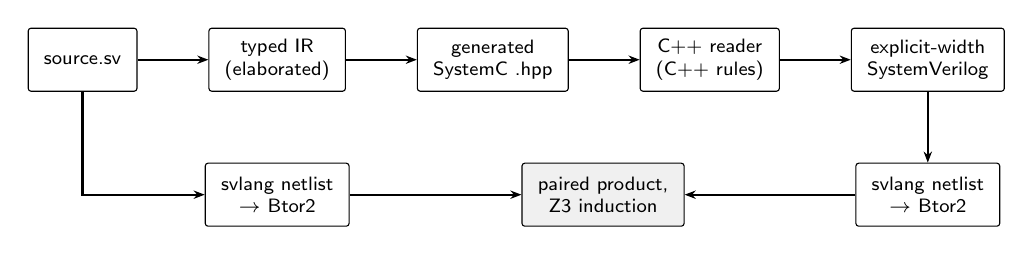
\begin{tikzpicture}[font=\sffamily\scriptsize,node distance=5mm and 9mm,
  box/.style={draw,rounded corners=1pt,align=center,minimum height=8mm,inner xsep=2mm,fill=white},
  arr/.style={-{Stealth[length=4pt]},thick}]
\node[box] (src) {source.sv};
\node[box,right=of src] (ir) {typed IR\\(elaborated)};
\node[box,right=of ir] (hpp) {generated\\SystemC .hpp};
\node[box,right=of hpp] (rd) {C++ reader\\(C++ rules)};
\node[box,right=of rd] (ew) {explicit-width\\SystemVerilog};
\node[box,below=9mm of ir] (net) {svlang netlist\\$\rightarrow$ Btor2};
\node[box,below=9mm of ew] (net2) {svlang netlist\\$\rightarrow$ Btor2};
\node[box,below=9mm of hpp,xshift=14mm,fill=black!6] (z3) {paired product,\\Z3 induction};
\draw[arr] (src) -- (ir);
\draw[arr] (ir) -- (hpp);
\draw[arr] (hpp) -- (rd);
\draw[arr] (rd) -- (ew);
\draw[arr] (src) |- (net);
\draw[arr] (ew) -- (net2);
\draw[arr] (net) -- (z3);
\draw[arr] (net2) -- (z3);
\end{tikzpicture}}
\caption{RTL conversion and proof in \code{svcc}. \code{rtl2sc} runs the top row as far as the
header; \code{rtl-prove} runs the rest. The reference side (left, bottom) never passes
through \code{svcc}'s intermediate representation. The other side starts from the bytes of the
generated header.}
\label{fig:arch}
\end{figure}

\emph{Conversion} (\code{rtl2sc}). \code{svlang} parses and elaborates the design, resolving
parameters and generate constructs, and binds every expression with the width and signedness
rules of IEEE~1800-2023. \code{svcc} lowers the result to one typed module per parameter set,
then emits one \code{SC\_MODULE} per module. The emitter keeps one invariant: every emitted C++
subexpression evaluates to exactly the value of its typed node, with an explicit truncation
wherever C++ would compute in a wider type. The supported subset follows what synthesis tools
accept~\cite{sutherland2014synth} and stays inside the IEEE~1666.1 synthesizable
subset~\cite{ieee1666_1_2016}: parameters, generate, hierarchy, functions, \code{case},
\code{casez} and \code{case inside}, loops, part selects, memories, packed structs and enums,
and vectors wider than 64 bits. Clock-gating cells, clock buffers and inverters are converted
into clock enables on the root clock, because a literal translation would run a delta cycle late.
Anything outside the subset is an error with a source location; \code{svcc} does not pass
unknown constructs through.

\emph{Proof} (\code{rtl-prove}). A purpose-built reader parses the generated header and gives
each expression the value C++17 gives it: integer promotion, the usual arithmetic conversions,
\code{sc\_uint} and \code{sc\_int} conversion to 64-bit integers, exact \code{sc\_biguint}
arithmetic. Operations whose result C++ does not define (signed overflow, division by zero,
out-of-range shifts and selects) raise a flag that the proof must show stays at zero. The reader
writes its result as SystemVerilog in which every width change is explicit, so SystemVerilog's
own context sizing cannot change it. Both that text and the original source are lowered by
\code{svlang} to Btor2, registers are paired by name, and Z3 proves by induction that outputs and
paired registers stay equal. If induction fails, a bounded check from reset is tried and the
result is labelled as bounded.

\emph{Golden models} (\code{prove-sec}). An untimed C++ function marked \code{// svcc:c2rtl}
can be proved equal to pipelined RTL \code{L} cycles later, from an arbitrary RTL state, in the
style of C-to-RTL equivalence checking~\cite{koelbl2009c2rtl}.

\emph{Co-simulation} (\code{rtl-cosim}). The generated SystemC and a Verilator model of the
same source are built into one executable and driven with the same random stimulus, comparing
every output after every step. This checks what the proof assumes, such as how a real SystemC
kernel schedules the code, and covers designs the proof does not.

\subsection{Software functionalities}

Table~\ref{tab:cli} lists the commands. Each exits with 0 on success, 1 on failure, and 3 when a
design is outside the proof model, so they can be used directly in scripts and continuous
integration.

\begin{table}[t]
\centering\small
\caption{Main \code{svcc} commands in version 0.1.0.}
\label{tab:cli}
\begin{tabularx}{\textwidth}{@{}l >{\raggedright\arraybackslash}X@{}}
\toprule
Command & Purpose \\
\midrule
\code{rtl2sc in.sv --top M} & Convert synthesizable RTL to a SystemC header \\
\code{rtl-prove in.sv [--header h]} & Prove the generated (or a given) header equal to the source \\
\code{rtl-cosim in.sv --top M} & Simulate the generated SystemC against Verilator \\
\code{prove-sec golden.hpp rtl.sv --latency L} & Prove a C++ golden function against pipelined RTL \\
\code{sv2sc}, \code{sc2sv}, \code{roundtrip-check} & Testbench path: UVM classes, constraints, covergroups and assertions \\
\bottomrule
\end{tabularx}
\end{table}

The Python package (\code{pip install svcc}) exposes the same operations as functions
(\code{rtl\_to\_sc}, \code{rtl\_prove\_json}, \code{prove\_sec\_json}, \code{sv\_to\_sc},
\code{sc\_to\_sv}), returning generated code or a JSON verdict. The Rust crate \code{svcc}
exposes them as a library.

The verdict of a proof is one of: \emph{proved} (by induction, for every run from equal
starting states), \emph{bounded} (no difference within a fixed number of steps), \emph{mismatch}
(with a concrete input sequence), \emph{inconclusive}, or \emph{not covered}. The documentation
(\code{docs/formal\_gates.md}) lists what the proof assumes: a two-state model in which X and Z
read as 0, \code{svlang} as the meaning of SystemVerilog, one clock with asynchronous reset seen
at the clock step, and \code{svcc}'s model of C++.

%% ---------------------------------------------------------------------------
\section{Illustrative examples}
\label{sec:examples}

The first example is the width rule from Section~\ref{sec:motivation}:

\begin{lstlisting}[language=Verilog]
module avg8(input [7:0] a, input [7:0] b, output [7:0] y);
  assign y = (a + b) >> 1;
endmodule
\end{lstlisting}

\noindent \code{svcc rtl2sc avg8.sv --top avg8} writes a header whose method truncates the sum
before the shift, as SystemVerilog does:

\begin{lstlisting}[language=C++]
void assign_y() {
  y.write(sc_dt::sc_uint<8>(sc_dt::sc_uint<8>(a.read() + b.read()) >> 1U));
}
\end{lstlisting}

\noindent \code{svcc rtl-prove avg8.sv} proves both the lowering and the generated C++ in
about 12~ms of solver time each. To see what the proof is for, remove the inner
\code{sc\_uint<8>(...)}, the form a hand translation or a naive translator produces, and pass
the edited header with \code{--header}:

\begin{lstlisting}
[PASS] lowering      'avg8': proved for all runs from equal start states
[FAIL] generated C++ 'avg8': DIFFERENCE FOUND
         step 0 a = #xff
         step 0 b = #xff
         step 0 spec y = #x7f
         step 0 imp  y = #xff
error: [rtl-prove] 'avg8' is not proved equal to its generated SystemC
\end{lstlisting}

\noindent The counterexample is the input that exposes the 64-bit sum. A check that compared
the translator's intermediate form with the source, or read the C++ with SystemVerilog's sizing
rules, would pass this header: that is how an earlier version of \code{svcc}'s own check was
fooled~\cite{kubavat2026rtltv}.

The second example, \code{testdata/rtl/fsm\_enum.sv}, is a two-process state machine with an
enumerated state type, a package function and an asynchronous reset. \code{rtl-prove} pairs its
two registers and proves the generated model by induction in about 12~ms. The third,
\code{testdata/rtl/clock\_gating.sv}, holds several gated clocks; \code{rtl2sc} converts them to
enables, but the design has more than one clock in the proof model, so \code{rtl-prove} reports
it as not covered, exits with code 3, and leaves co-simulation as the evidence.

%% ---------------------------------------------------------------------------
\section{Impact}
\label{sec:impact}

\emph{A checked model instead of a trusted one.} The main use is to give a design or
verification team a SystemC model of its RTL that comes with a proof, or, where the proof does
not reach, with a labelled reason and simulation evidence. Because the proof reads the C++ and
not the translator's intent, it can also check C++ that \code{svcc} did not write, provided it
stays in the subset the reader models. That includes output from a language model asked to
translate RTL, which is an open research question this tool makes measurable.

\emph{Evidence on real designs.} In the companion study~\cite{kubavat2026rtltv}, every module of
15 open-source designs (among them OpenTitan, CVA6, Ibex, cv32e40p and Caliptra; 2,184 modules)
was tried as a top. 1,185 of them were converted to SystemC that compiles and matches Verilator
over 3,000 random steps; the rest are rejected with a located error or listed with the cause of
the difference. % NUMBERS: journal entry M5.2-clock-gating (2026-11-23); refresh before submission.
On the 50 designs of the repository, the proof covers 45 by induction and reports the other 5 as
not covered (several clocks or a multi-dimensional array port), and in a mutation
experiment no mutant that simulation showed to be wrong was accepted by the proof.

\emph{A differential test harness for other tools.} Running one design through \code{svlang},
\code{svcc}, SystemC and Verilator and comparing them tests all four. During the study it found
three defects in \code{svlang}'s elaboration (a dropped generate branch, a fill literal read as
1, a mis-bound struct member select), which were fixed in \code{svlang}~0.5.1, as well as cases
where Verilator's result was the questionable one. This continues the line of differential
testing of compilers~\cite{yang2011csmith} and synthesis tools~\cite{herklotz2020verismith}.

\emph{Golden-model checking.} \code{prove-sec} found undefined behaviour in one of
\code{svcc}'s own benchmark golden models (a 16-bit product computed in \code{int}), the kind of
error that passes testing on a given compiler.

\emph{Adoption.} Version 0.1.0 was published to crates.io and PyPI on 22 November 2026. It is
too early to report outside users. % TODO: add download counts, issues or users at submission time if any.

%% ---------------------------------------------------------------------------
\section{Conclusions}
\label{sec:conclusions}

\code{svcc} converts synthesizable SystemVerilog to readable SystemC and proves each result
equal to its source by reading the C++ with C++ rules. It is explicit about the limits of that
proof: one clock, two-state values, a synchronous view of asynchronous reset, and a model of C++
rather than a compiler front end. Planned work is to extend the proof to several clocks, to run
it on the full real-design corpus, and to give the testbench path (UVM-SystemC, CRAVE and FC4SC)
checks of the same strength.

\section*{Declaration of competing interest}
The author declares no competing financial interests or personal relationships that could have
appeared to influence the work reported in this paper. The work was done independently, on
personal equipment, and is not affiliated with or endorsed by any employer.

\section*{Declaration of generative AI and AI-assisted technologies in the writing process}
% Check the wording against the current Elsevier template before submission.
During the preparation of this work the author used AI coding and writing assistants to draft
parts of the software, test scripts and this manuscript. The author reviewed and edited all
generated material, ran every command and measurement reported here, and takes full
responsibility for the content of the publication.

\section*{Acknowledgements}
The author thanks the maintainers of Verilator, SystemC and Z3.

\bibliographystyle{elsarticle-num}
\bibliography{refs}

\end{document}
